\newpage
\section{Using the Integrator}
\genHeader
\label{sec:app_integrator}

Let's check out another model visualization feature of eMolfon, the integrator! While you can ``see" the structure of a model with the graph viewer, the
integrator allows you to trace the transformation process. In other words, the integrator works as an ``offline'' debugger, working on the protocol (trace) of
the transformation.

\begin{itemize}

\item[$\blacktriangleright$] Right-click on \texttt{corr\_BWD.xmi} and choose ``eMoflon $\rightarrow$ Start Integrator'' which will open the window depicted in
Fig.~\ref{fig:integrator_start}.

\vspace{0.5cm}

\begin{figure}[htbp]
\begin{center}
  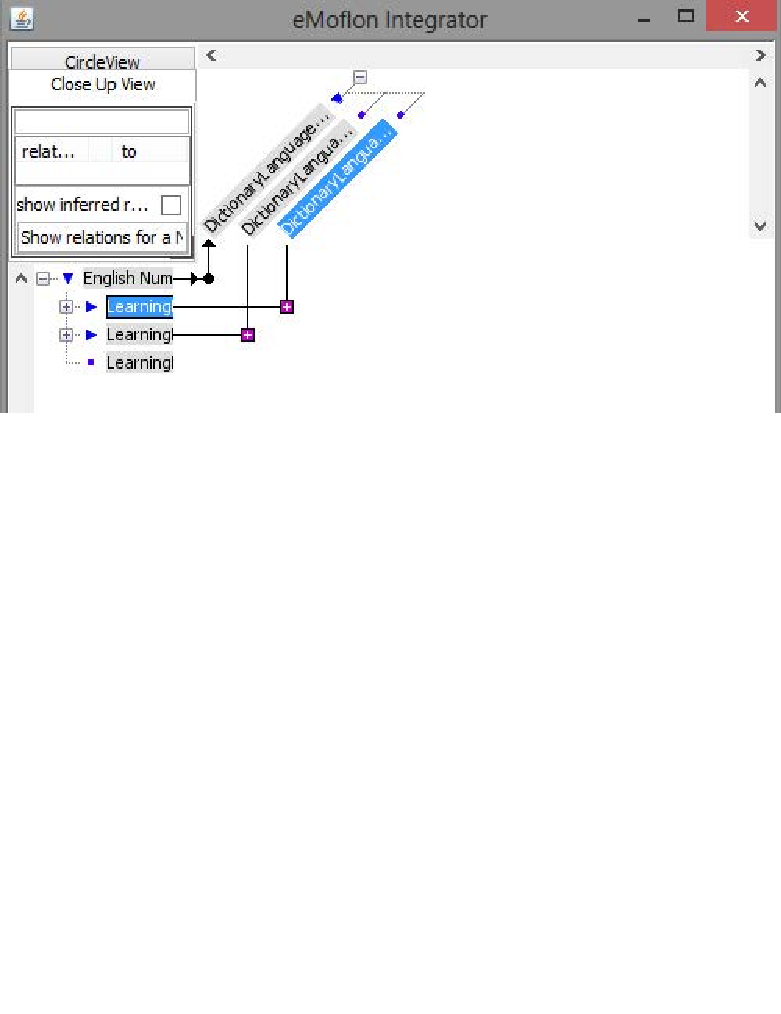
\includegraphics[width=0.7\textwidth]{integrator_start_view.pdf}
  \caption{Default view of the integrator}
  \label{fig:integrator_start}
\end{center}
\end{figure}

\item[$\blacktriangleright$] Drag and drop \texttt{protocol\_BWD.xmi} into the main window.\footnote{If the integrator window minimizes, press \texttt{alt+tab}
to re-activate it} You will now see the navigation controls explained in the lower part of the window (Fig.~\ref{fig:integrator_after_protocol}).

\vspace{0.5cm}

\item[$\blacktriangleright$]  Starting at \texttt{Box}, you can use \texttt{Alt+Right} to navigate forwards \emph{through} the transformation process, and
\texttt{Alt+Left} to go backwards -- each step will appear with a small explanation in the small window below.

\item[$\blacktriangleright$] It should begin with the statement \texttt{Starting translation protocol}. It will then state what \texttt{node} is now active,
then list the possible rule candiates. The goal of this process is to check \emph{every} possible action with every applicable item. Given that you only have
one rule that deals with partitions, this list will be short and will perform the operation. Before moving on to the next node, it will state wether or not the
operation was successful.

\newpage

\begin{figure}[h!]
\begin{center}
  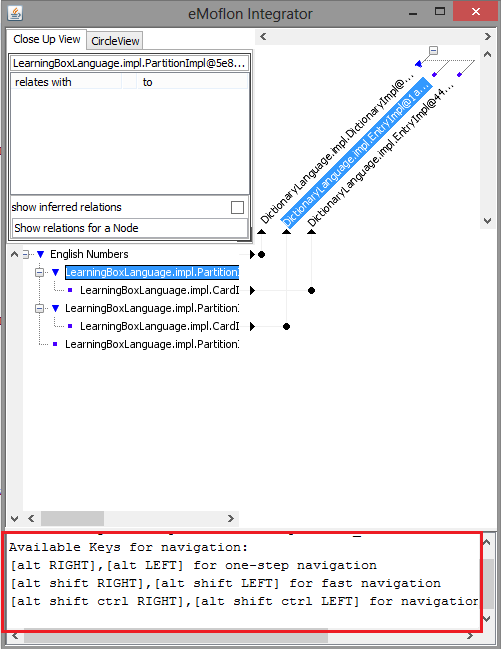
\includegraphics[width=0.6\textwidth]{integrator_after_protocol_insertion.png}
  \caption{Integrator after protocol insertion.}
  \label{fig:integrator_after_protocol}
\end{center}
\end{figure} 

\item[$\blacktriangleright$] While you're stepping through the transformation, you'll notice that some elements become highlighted with different colours. They
represent the elements currently being processed, and each have the following definitions:

\begin{description}
  \item[Blue] The element is currently being ``looked at," and is about to be processed.
  
  \vspace{0.5cm}
  
  \item[Yellow] The element cannot be transformed right now and has been queued for later transformation (i.e., when transforming the first
  \texttt{Entry} into a \texttt{Card}, the \texttt{Box} with each \texttt{partition} to store \texttt{card} must be translated first); ``Paused.''
  
  \vspace{0.5cm}
  
  \item[Green] The object has been created.

\end{description}

\end{itemize}
